\documentclass[twoside]{article}
\usepackage{amsgen,amsmath,amstext,amsbsy,amsopn,amssymb,comment}
\usepackage[export]{adjustbox}
\usepackage{graphicx}
\usepackage{epsfig}

\setlength{\oddsidemargin}{-1 in} \setlength{\evensidemargin}{-1in} 
\setlength{\topmargin}{-1 in} \setlength{\textwidth}{7.7 in}
\setlength{\textheight}{10.4 in} \setlength{\headsep}{0.1 in}
\setlength{\parindent}{0 in} \setlength{\parskip}{0.1 in}

\newcommand{\homework}[2]{
   \pagestyle{myheadings}
   \thispagestyle{plain}
   \newpage
   \setcounter{page}{1}
   \noindent
   \begin{center}
   \framebox{
      \vbox{\vspace{2mm}
       \hbox to 6.28in { {\bf Math 4720:~Exam 1 \hfill} }
       \vspace{6mm}
       \hbox to 6.28in { {\Large \hfill #1 (#2)  \hfill} }
       \vspace{6mm}
      \vspace{2mm}}
   }
   \end{center}
   \markboth{#1}{#1}
   \vspace*{4mm}
}

\newcommand{\bbF}{\mathbb{F}}
\newcommand{\bbX}{\mathbb{X}}
\newcommand{\bI}{\mathbf{I}}
\newcommand{\bX}{\mathbf{X}}
\newcommand{\bY}{\mathbf{Y}}
\newcommand{\bepsilon}{\boldsymbol{\epsilon}}
\newcommand{\balpha}{\boldsymbol{\alpha}}
\newcommand{\bbeta}{\boldsymbol{\beta}}
\newcommand{\0}{\mathbf{0}}

\begin{document}

\begin{comment}
\homework{Formula Sheet}{08/31/14}
\vspace{-.3in}
\begin{itemize}
\item Measure of the center
\subitem \textbf{Mean} : $\bar{x}=\dfrac{1}{n}\sum_{i=1}^nx_i$,\ \ \ \ \ \textbf{Median}
\item Five number summary : Min, Q1, Median, Q3, Max
\item Measure of Spread
\subitem Variance : $s^2=\dfrac{1}{n-1}\sum_{i=1}^n(x_i-\bar{x})^2$, Standard deviation : $s=\sqrt{s^2}$
\subitem IQR : $IQR = Q3 - Q1$
\item Correlation $r=\dfrac{1}{n-1}\sum_{i=1}^n\Biggl(\dfrac{x_i-\bar{x}}{s_x}\Biggr)\Biggl(\dfrac{y_i-\bar{y}}{s_y}\Biggr)$
\item If $A$ and $B$ are disjoint, $P(A \ \textrm{or} \ B) = P(A \bigcup B) = P(A) + P(B)$
\item For any event $A$, $P(A$ does not occur$) = P(\bar{A}) = 1 - P(A)$.
\item Addition rule in general : $P(A \ \textrm{or} \ B) = P(A \bigcup B) = P(A) + P(B) - P( A \bigcap B )$
\item The conditional probability of A given B is: $P(A|B) = \dfrac{P(A \ \textrm{and} \ B)}{P(B)} = \dfrac{P(A \bigcap B)}{P(B)}$
\item General \textbf{multiplication} rule : $P(A \ \textrm{and} \ B) = P(A \bigcap B) = P(A|B) P(B) = P(B|A) P(A)$.
\item Two events $A$ and $B$ are \textbf{independent} if: $P(A|B) = P(A)$ or $P(A \bigcap B)=P(A)P(B)$.
\item Bayes' Rule : Suppose that $A_1, A_2, \ldots, A_k$ are disjoint events whose probabilities add to exactly 1, then:
    $$P(A_i|B)=\dfrac{P(B|A_i)P(A_i)}{P(B|A_1)P(A_1)+\ldots+P(B|A_k)P(A_k)}$$
\tem \textbf{Binomial$(n,\pi)$}: $P(X=k)=\dfrac{n!}{k!(n-k)!}\pi^k(1-\pi)^{n-k}$, $k=0,1,2,\cdots,n$
\item \textbf{Poisson$(\mu)$}: $P(Y=y)=\dfrac{\mu^ye^{-\mu}}{y!}$, $y=1,2,\cdots$
\item The standardized value is called a z-score. $z=\dfrac{x-\mu}{\sigma}$
\item Finding Normal Probabilities :
\subitem Less than: $P(X<x)=P\Bigl(\dfrac{X-\mu}{\sigma}<\dfrac{x-\mu}{\sigma}\Bigr)=P(Z<z)$
\subitem Greater than: $P(X>x)=P(Z>z)=1-P(Z<z)$
\subitem Between two numbers: $P(a<X<b)=P(z_a<Z<z_b)=P(Z<z_b)-P(Z<z_a)$
\subitem $P(X < a \bigcup X > b)=P(Z < z_a \bigcup Z > z_b)=1-P(z_a<Z<z_b)=P(Z<z_a)+1-P(Z<z_b)$
\item \textbf{CLT} (Central Limit Theorem): Draw a random sample of size $n$ from any population with mean $\mu$ and finite standard deviation $\sigma$. When $n$ is large, the sampling distribution of the sample mean is approximately $N(\mu,\dfrac{\sigma^2}{n})$.
\item Confidence interval : $\textrm{estimate} \pm \textrm{margin of error}$. A confidence interval for $\mu$ is $\bar{x} \pm z_{\alpha/2}\dfrac{\sigma}{\sqrt{n}}$
\item The confidence interval will have a specified \textbf{margin of error} $E$ when the sample size is: $n=\Bigl(\dfrac{z_{\alpha/2}\sigma}{E}\Bigr)^2$
\end{itemize}
\newpage
\end{comment}

\vspace{-1.5in}
\begin{itemize}
\item[] \textbf{Formula Sheet\hspace{6.3cm} Math 4720\hspace{6.4cm} Exam 2}
\item \textbf{CLT} (Central Limit Theorem): Draw a random sample of size $n$ from any population with mean $\mu$ and finite standard deviation $\sigma$. When $n$ is large, the sampling distribution of the sample mean is approximately $N(\mu,\dfrac{\sigma^2}{n})$.
\item Confidence interval : $\textrm{estimate} \pm \textrm{margin of error}$. A confidence interval for $\mu$ is $\bar{x} \pm z_{\alpha/2}\dfrac{\sigma}{\sqrt{n}}$
\item The confidence interval will have a specified \textbf{margin of error} $E$ when the sample size is: $n=\Bigl(\dfrac{z_{\alpha/2}\sigma}{E}\Bigr)^2$
\item A \textbf{test statistic} calculated from the sample data measures how far the data diverge from the null hypothesis $H_0$. Define the test statistic $z=\dfrac{\bar{x}-\mu_0}{\sigma/\sqrt{n}}$
\subitem Decision Rule: Given fixed $\alpha=P(\textrm{Type-I Error})$.
\subsubitem $H_a: \mu > \mu_0$, Reject $H_0$ if $z>z_{\alpha}$
\subsubitem $H_a: \mu < \mu_0$, Reject $H_0$ if $z<-z_{\alpha}$
\subsubitem $H_a: \mu \neq \mu_0$, Reject $H_0$ if $|z|>z_{\alpha/2}$
\item If we reject $H_0$ when in fact $H_0$ is true, this is a \textbf{Type I error}.
\item If we fail to reject $H_0$ when in fact $H_a$ is true, this is a \textbf{Type II error}, also called $\beta$.
\subitem For one sided alternative test ($H_a:\mu>\mu_0$ or $H_a:\mu<\mu_0$ ): $\beta=P\Bigl(Z\leq z_\alpha-\dfrac{|\mu_0-\mu_a|}{\sigma/\sqrt{n}}\Bigr)$
\subitem For two sided alternative test ($H_a:\mu \neq \mu_0$): $\beta=P\Bigl(Z\leq z_{\alpha/2}-\dfrac{|\mu_0-\mu_a|}{\sigma/\sqrt{n}}\Bigr)$
\item \textbf{Power analysis} (Sample size determination), where power $= 1 - \beta$:
\subitem For one sided alternative test ($H_a:\mu>\mu_0$ or $H_a:\mu<\mu_0$ ): $n=\sigma^2\dfrac{(z_\alpha+z_\beta)^2}{\Delta^2}$
\subitem For two sided alternative test ($H_a:\mu \neq \mu_0$): $n=\sigma^2\dfrac{(z_{\alpha/2}+z_\beta)^2}{\Delta^2}$
\item The \textbf{one-sample t statistic}: $t=\dfrac{\bar{x}-\mu}{s/\sqrt{n}}$ has the \textbf{t distribution} with $n-1$ degrees of freedom.
\subitem The p\_value for a test of $H_0: \mu = \mu_0$ vs
\subsubitem $H_a: \mu > \mu_0$ is p-value $ = P(T\geq t)$
\subsubitem $H_a: \mu < \mu_0$ is p-value $ = P(T\leq t)$
\subsubitem $H_a: \mu \neq \mu_0$ is p-value $ = 2P(|T|\geq|t|)$
\item Confidence interval for $\mu$ is:
\subitem $\bar{x} \pm t_{\alpha/2}\dfrac{s}{\sqrt{n}}$ with $df=n-1$
\end{itemize}
\vspace{-4cm}
\begin{figure}[h]
\hspace{2cm}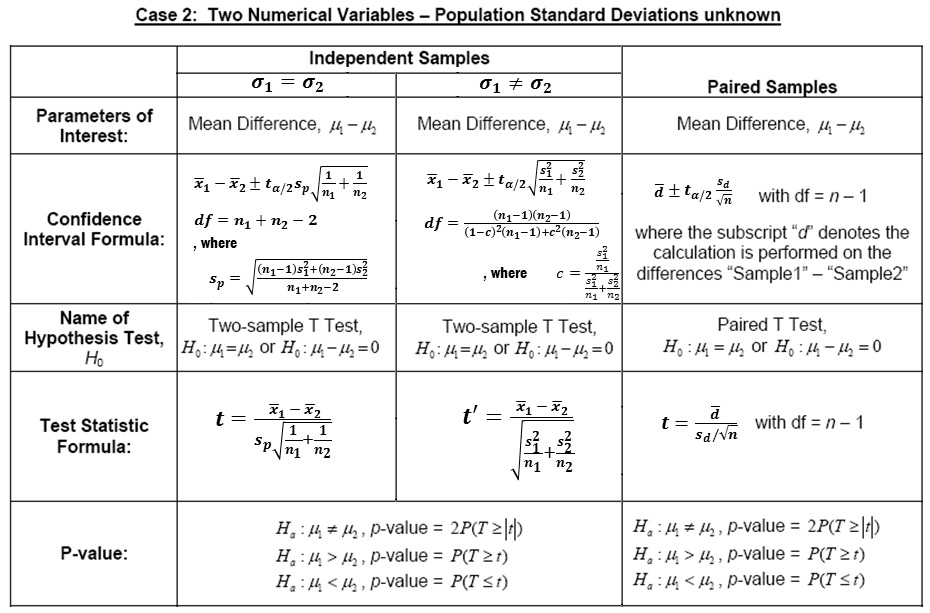
\includegraphics[width=.7\textwidth,right]{HT_3.jpg}
\end{figure}
\vspace{-5.5cm}
\begin{itemize}
\vspace{-0.25cm}
\item \textbf{Power analysis} (2 Independent Samples):
\subitem for ($H_a:\mu_1>\mu_2$ or $H_a:\mu_1<\mu_2$ ): 
\subsubitem $n=\dfrac{2\sigma^2(z_\alpha+z_\beta)^2}{\Delta^2}$
\subitem for ($H_a:\mu_1 \neq \mu_2$): 
\subsubitem $n=\dfrac{2\sigma^2(z_{\alpha/2}+z_\beta)^2}{\Delta^2}$
\item \textbf{Power analysis} (Paired Samples):
\subitem for ($H_a:\mu_1>\mu_2$ or $H_a:\mu_1<\mu_2$ ): 
\subsubitem $n=\dfrac{\sigma_d^2(z_\alpha+z_\beta)^2}{\Delta^2}$
\subitem for ($H_a:\mu_1 \neq \mu_2$): 
\subsubitem $n=\dfrac{\sigma_d^2(z_{\alpha/2}+z_\beta)^2}{\Delta^2}$
\vspace{.25cm}
\item \textbf{NON-PARAMETRIC TESTS:} For the population median: use SIGN TEST. For TWO Independent Samples: use WILCOXON RANK-SUM TEST. For TWO Dependent Samples: use WILCOXON SIGNED-RANK TEST
\end{itemize}
\end{document}
